% Main file, compiler: XeLaTeX.
\documentclass[a4paper,12pt]{article}
\usepackage{fontspec,polyglossia}
\setmainlanguage{russian}
\setotherlanguage{english}
\IfFontExistsTF{DejaVu Serif}{\setmainfont{DejaVu Serif}}{\setmainfont{Times New Roman}}
\IfFontExistsTF{DejaVu Sans}{\setsansfont{DejaVu Sans}}{\setsansfont{Arial}}
\IfFontExistsTF{DejaVu Sans Mono}{\setmonofont{DejaVu Sans Mono}}{\setmonofont{Consolas}}
\usepackage{amsmath,amssymb}
\usepackage[left=25mm,right=20mm,top=20mm,bottom=22mm]{geometry}
\usepackage{graphicx,float,booktabs,tabularx,longtable}
\usepackage{caption,subcaption,fancyhdr}
\usepackage[hidelinks]{hyperref}
\usepackage{xurl}
\hypersetup{hypertexnames=false}
\setlength{\parindent}{1.25cm}
\setlength{\parskip}{0.2em}
\setlength{\headheight}{15pt}
\emergencystretch=3em
\renewcommand{\arraystretch}{1.15}
\captionsetup{font=small,labelfont=bf}
\pagestyle{fancy}\fancyhf{}
\fancyhead[L]{\small Алгоритмы компьютерной графики}
\fancyhead[R]{\small Лабораторная работа № 4}
\fancyfoot[C]{\thepage}
\renewcommand{\headrulewidth}{0pt}
\newcommand{\code}[1]{\nolinkurl{#1}}
\begin{document}
\begin{titlepage}\thispagestyle{empty}
\begin{center}
\textbf{МИНИСТЕРСТВО НАУКИ И ВЫСШЕГО ОБРАЗОВАНИЯ РФ}\\[0.6em]
\textbf{УНИВЕРСИТЕТ ИТМО}\\[0.6em]
Факультет программной инженерии и компьютерной техники
\vfill
{\Large\bfseries ОТЧЁТ ПО ЛАБОРАТОРНОЙ РАБОТЕ № 4}\\[1.2em]
{\large по дисциплине «Алгоритмы компьютерной графики»}\\[2em]
{\Large\bfseries Моделирование цветных изображений\\[0.35em]
Построение спектра по цвету}
\vfill
Выполнили: Чжун Ц. Чэнь Х.\\
Группы: P3310, P3316\\
Преподаватель: Потемин Игорь Станиславович
\vfill Санкт-Петербург\\2026
\end{center}\end{titlepage}
\tableofcontents\clearpage

\section{Цель и постановка задачи}
Цель работы --- построить спектральное представление сцены по её координатам RGB и сформировать изображение белой диффузной сферы, освещённой точечными источниками с ламбертовской диаграммой излучения.

Часть A: RGB сцены $\to$ спектры источников и материала $\to$ абсолютное спектральное изображение $\to$ абсолютное RGB изображение $\to$ мониторный файл \code{image_A.png}. В части B сравниваются исходные и восстановленные спектры таблицами и графиками. В части C изображение A сравнивается с \code{image_1} и \code{image_2} лабораторной работы 3. Прилагаются код, изображения, абсолютная яркость в трёх точках и экстремумы на сфере.

Экран имеет размеры 100--10000 мм по каждой стороне. Разрешение по каждой стороне --- 200--800 пикселей с квадратным пикселем. Координаты источников лежат в пределах $\pm10000$ мм, центр сферы имеет $x_C,y_C\in[-10000,10000]$ мм и $z_C\in[0,10000]$ мм. Наблюдатель расположен в $(0,0,z_O)$, сфера целиком помещается в поле зрения. Исходная интегральная сила излучения $I_0$ находится в диапазоне 0,01--10000 Вт/ср. Спектральная сетка --- 380--780 нм с шагом 10 нм.

\section{Использованные учебные материалы}
Теория и алгоритм сверены со следующими материалами курса:
\begin{enumerate}
\item Жданов Д.Д., Потемин И.С., Жданов А.Д. \emph{Теоретические основы компьютерной графики и вычислительной оптики}, 2023, файл \code{3281.pdf}. С.~47, формула (3.4.5.1) задаёт ламбертовское отражение. Раздел 4.2, с.~64--66, объясняет аддитивность, метамерию и восстановление спектра на примере D65. С.~70 содержит числовую матрицу CIE RGB $\to$ XYZ, с.~77 --- матрицу XYZ $\to$ линейный sRGB.
\item Лекция 4 А. Игнатенко, \code{mis_lect04_11.pdf}, с.~35--42 PDF. На с.~37--41 дана последовательность RGB $\to$ XYZ $\to$ три базовых спектра $\to$ решение системы коэффициентов. С.~42 допускает непрерывные базисные функции и указывает возможность отрицательного результата.
\item Лекция 5, \code{mis_lect05_11.pdf}, с.~43--46 PDF: расчёт в линейном представлении и мониторная гамма 2,2. Лекция 3, с.~46--47 PDF: отображение цветового охвата.
\end{enumerate}
У пособия печатный номер страницы меньше номера страницы PDF на единицу. Метод максимальной энтропии и ограничение единичной энергии при восстановлении не применяются, поскольку они не входят в выбранную учебную последовательность.

\section{Исходная сцена}
Геометрия, таблицы CIE XYZ и D65 взяты из лабораторной работы 3. Как требует работа 4, материал заменён на белый: $k_d(\lambda)=1$, $k_d^{RGB}=(1,1,1)$. Цвет источников заново выражен в согласованной паре матриц учебника.
\begin{table}[H]\centering\small
\caption{Параметры основного опыта}
\begin{tabularx}{\textwidth}{@{}lX@{}}\toprule
Параметр & Значение\\\midrule
Экран & $1200\times1200$ мм, $600\times600$ пикселей, $z=0$\\
Наблюдатель & $(0,0,2500)$ мм, направление $(0,0,-1)$\\
Сфера & $C=(0,0,600)$ мм, $R=350$ мм\\
Источник 1 & $(-650,450,1700)$ мм, $I_0=100$ Вт/ср\\
Источник 2 & $(550,-250,1600)$ мм, $I_0=70$ Вт/ср\\
Оси источников & $(0,0,-1)$\\
Исходные спектры & D65 с единичным интегралом\\\bottomrule
\end{tabularx}\end{table}
\begin{table}[H]\centering\small
\caption{CIE RGB исходных относительных спектров}
\begin{tabular}{@{}lrrr@{}}\toprule Источник & R & G & B\\\midrule
L1 & 0.2526108113 & 0.3104552518 & 0.3269916595 \\
L2 & 0.2526108113 & 0.3104552518 & 0.3269916595 \\
\bottomrule\end{tabular}\end{table}
RGB означает линейные CIE RGB 1931, а не коды изображения 0--255. Функции стандартного наблюдателя взяты из преподавательской таблицы. Для интегрирования приняты трапецеидальные веса $w_0=w_{40}=5$ нм и $w_j=10$ нм внутри диапазона. Это численная дискретизация интеграла учебника под сетку задания.

\clearpage
\section{Алгоритм построения спектра по RGB}
\subsection{Переход в XYZ}
По числовой матрице пособия на с.~70:
\[
 \boldsymbol X=M\boldsymbol R,\qquad
 M=\begin{pmatrix}
 .49&.31&.20\\ .17697&.81240&.01063\\ 0&.01&.99
 \end{pmatrix},\quad \boldsymbol R=(R,G,B)^T.
\]
Обратная матрица вычисляется как $M^{-1}$, а не берётся из независимо округлённой таблицы. Цветовые интегралы:
\[
 X=\sum_jw_js_j\bar x_j,\qquad Y=\sum_jw_js_j\bar y_j,\qquad
 Z=\sum_jw_js_j\bar z_j.
\]

\subsection{Три базовых спектра}
Согласно лекции 4, с.~39 и 42, базис задаётся тремя линейно независимыми функциями. На с.~66 пособия, рис.~4.6, показана реконструкция D65 через кривые стандартного наблюдателя. Выбран соответствующий непрерывный базис:
\[
 F_1(\lambda)=\bar x(\lambda),\quad F_2(\lambda)=\bar y(\lambda),\quad
 F_3(\lambda)=\bar z(\lambda),\qquad S(\lambda)=\sum_{k=1}^3a_kF_k(\lambda).
\]
Это конкретный выбор из разрешённого лекцией класса функций. Он зафиксирован в программе, переключателя методов нет.

\subsection{Решение системы}
Пусть $F$ --- матрица $41\times3$ значений базиса, а $T$ --- матрица $3\times41$ цветовых интегралов, строки которой равны $w_j\bar x_j$, $w_j\bar y_j$, $w_j\bar z_j$. Подстановка в интегралы даёт
\[
 \boldsymbol X=C\boldsymbol a,\quad C=TF,\qquad
 C_{ik}=\sum_jw_j\bar c_i(\lambda_j)F_k(\lambda_j).
\]
Лекция записывает $\boldsymbol a=C^{-1}M\boldsymbol R$. В коде эквивалентная система $C\boldsymbol a=M\boldsymbol R$ решается функцией \code{numpy.linalg.solve}, затем $\boldsymbol s=F\boldsymbol a$. Исходный D65 не передаётся функции восстановления и нужен только для получения входного RGB и сравнения.

Матрица строится по интегральным определениям с.~40 лекции. На с.~41 в третьей строке рисунка повторён индекс длины волны. В программе столбцы соответствуют своим базисным функциям, как следует из интегралов предыдущей страницы.

\subsection{Физические ограничения и энергия}
Лекция 4 указывает, что метод может дать отрицательный спектр. В этом случае приложение сообщает об ошибке. Спектр не обрезается, базис не меняется и другой решатель не подключается.

Система сохраняет XYZ и RGB, но не задаёт $\int S\,d\lambda$. Поэтому восстановленный спектр не нормируется повторно. Исходный относительный спектр имеет интеграл 1, после восстановления интеграл может измениться. Фактическая интегральная сила излучения восстановленного источника:
\[
 I_{i,\mathrm{reconstructed}}=I_{0i}\sum_jw_js_{ij}.
\]
$I_{0i}$ остаётся масштабом исходной сцены. Деление реконструкции на её интеграл изменило бы заданные абсолютные цветовые координаты. Белый материал восстанавливается по известному условию отсутствия спектральной избирательности: $k_d(\lambda)=1$. Проверка $RGB(D65\cdot k_d)/RGB(D65)$ даёт $(1,1,1)$.

\section{Расчёт яркости и изображения}
Камера использует центры пикселей и перспективные лучи. Уравнения луча и сферы сверены с лекцией 11, с.~34--35 PDF. Для луча $P=O+t\boldsymbol q$, $\|\boldsymbol q\|=1$, пересечение со сферой определяется из
\[
 b=\boldsymbol q\cdot(O-C),\quad c=\|O-C\|^2-R^2,\quad
 D=b^2-c,\quad t=-b-\sqrt D.
\]
Выбирается ближайшее положительное пересечение, фон отмечается независимой маской. Проверяются радиус, полный силуэт в поле зрения, квадратность пикселя и размещение наблюдателя и источников вне сферы.

Для точки $P$ нормаль направлена наружу. Пусть $\boldsymbol l_i$ --- единичный вектор от поверхности к источнику, $\boldsymbol a_i$ --- единичная ось источника, $r_i$ --- расстояние в метрах. Вычисляются
\[
 c_{\theta i}=\max(-\boldsymbol a_i\cdot\boldsymbol l_i,0),\qquad
 c_{\sigma i}=\max(\boldsymbol n\cdot\boldsymbol l_i,0).
\]
Диаграмма источника задаёт $I_i=I_{0i}c_{\theta i}$, закон освещённости --- $E_i=I_ic_{\sigma i}/r_i^2$. По формуле (3.4.5.1) пособия $L=k_dE/\pi$:
\[
 L_{\lambda_j}(P)=\sum_i\frac{I_{0i}c_{\theta i}c_{\sigma i}}
 {\pi r_i^2}s_{ij}k_{dj}.
\]
Приёмный косинус входит один раз. Дополнительная степень косинуса прежней реализации исключена. Зеркальный член, фоновое освещение и многократные отражения не добавляются.

В памяти хранится float64 массив $H_{res}\times W_{res}\times41$ в Вт/(м$^2\cdot$ср$\cdot$нм). Из него вычисляются XYZ, CIE RGB и
\[
 L_e=\sum_jw_jL_{\lambda_j},\qquad L_v=683Y\quad[\text{кд/м}^2].
\]
Для вывода применяется матрица XYZ $\to$ линейный sRGB пособия, с.~77. Три изображения делятся на общий положительный максимум каналов, ограничиваются диапазоном $[0,1]$, затем по лекции 5 применяется гамма 2,2: $v_{out}=v_{linear}^{1/2.2}$. Результат округляется как $\operatorname{round}(255v_{out})$. Это учебное приближение мониторной гаммы, а не точная кусочная функция sRGB. Абсолютные массивы сохраняются до этих операций.

\clearpage
\section{Результаты}
\subsection{Спектры источников и материала}
\begin{figure}[H]\centering
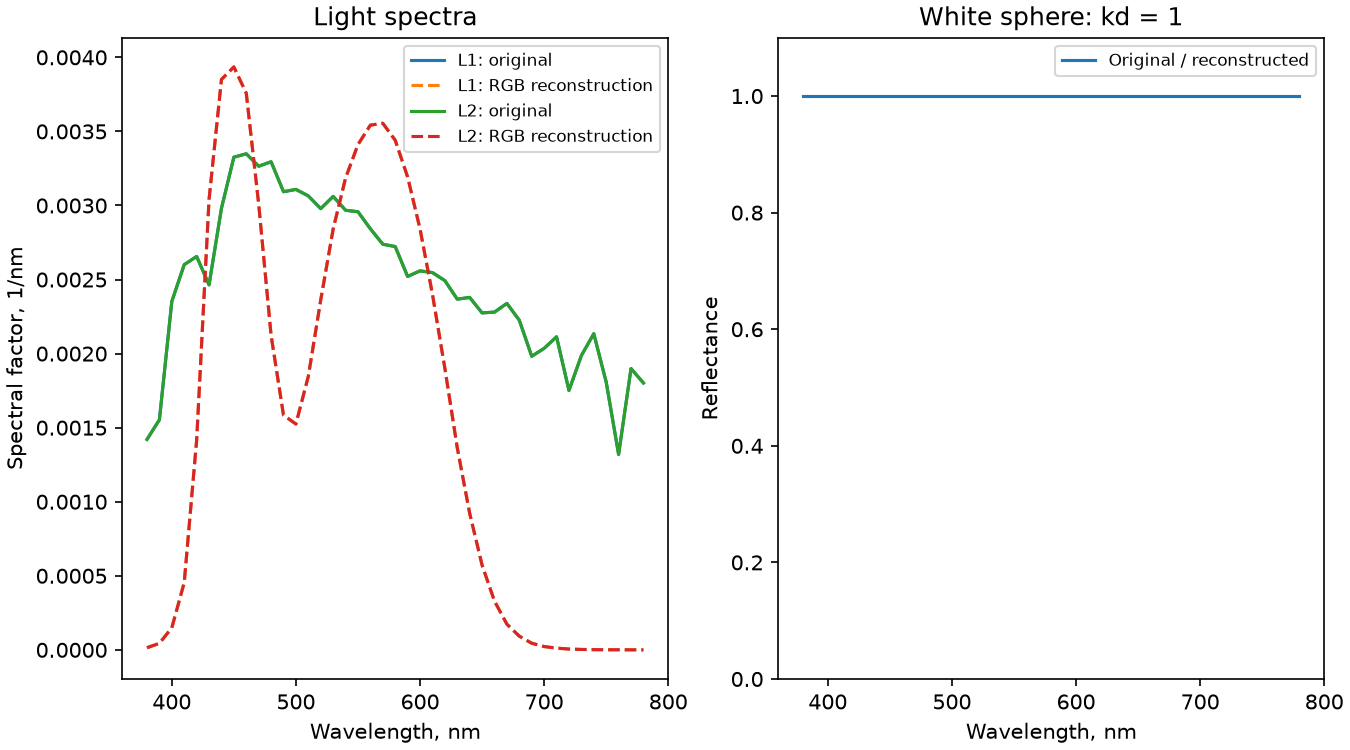
\includegraphics[width=\textwidth]{figures/spectra_comparison.png}
\caption{D65 и результаты трёхбазисной реконструкции}
\end{figure}
Оба источника имеют одинаковый цвет, поэтому их относительные реконструкции совпадают. Различаются положение и входной масштаб $I_0$. Белый материал имеет нулевую ошибку во всех 41 отсчётах.
RMSE формы спектра равна 0.0014188447 нм$^{-1}$, максимальная ошибка --- 0.0022034809 нм$^{-1}$. Ошибка обратного RGB не превышает $1.11\cdot10^{-16}$. Интеграл реконструкции равен 0.6295556600 вместо исходного 1. Интегральные силы излучения реконструированных источников составляют 62.95556600 и 44.06889620 Вт/ср.

\begin{longtable}{@{}rrrr@{}}
\caption{Спектральные множители L1 и L2, одинаковые для обоих источников, нм$^{-1}$}\\
\toprule $\lambda$, нм & Исходный & Восстановленный & Разность\\\midrule\endfirsthead
\toprule $\lambda$, нм & Исходный & Восстановленный & Разность\\\midrule\endhead
380 & 0.00142056 & 0.00001416 & -0.00140640 \\
390 & 0.00155338 & 0.00004397 & -0.00150940 \\
400 & 0.00235231 & 0.00014883 & -0.00220348 \\
410 & 0.00260049 & 0.00045438 & -0.00214611 \\
420 & 0.00265580 & 0.00141433 & -0.00124147 \\
430 & 0.00246395 & 0.00304063 & +0.00057668 \\
440 & 0.00298079 & 0.00385085 & +0.00087006 \\
450 & 0.00332596 & 0.00393550 & +0.00060954 \\
460 & 0.00334881 & 0.00375773 & +0.00040892 \\
470 & 0.00326493 & 0.00300892 & -0.00025601 \\
480 & 0.00329512 & 0.00212271 & -0.00117241 \\
490 & 0.00309296 & 0.00158410 & -0.00150886 \\
500 & 0.00310839 & 0.00152444 & -0.00158395 \\
510 & 0.00306428 & 0.00184730 & -0.00121698 \\
520 & 0.00297866 & 0.00236257 & -0.00061609 \\
530 & 0.00306107 & 0.00284083 & -0.00022024 \\
540 & 0.00296772 & 0.00318514 & +0.00021742 \\
550 & 0.00295751 & 0.00341121 & +0.00045370 \\
560 & 0.00284251 & 0.00354237 & +0.00069986 \\
570 & 0.00273830 & 0.00355486 & +0.00081656 \\
580 & 0.00272278 & 0.00344025 & +0.00071747 \\
590 & 0.00252089 & 0.00319269 & +0.00067179 \\
600 & 0.00255843 & 0.00284160 & +0.00028317 \\
610 & 0.00254686 & 0.00240065 & -0.00014621 \\
620 & 0.00249284 & 0.00190128 & -0.00059156 \\
630 & 0.00236748 & 0.00136418 & -0.00100330 \\
640 & 0.00237915 & 0.00092155 & -0.00145760 \\
650 & 0.00227477 & 0.00057188 & -0.00170288 \\
660 & 0.00228010 & 0.00032889 & -0.00195121 \\
670 & 0.00233875 & 0.00017331 & -0.00216544 \\
680 & 0.00222523 & 0.00009240 & -0.00213284 \\
690 & 0.00198183 & 0.00004468 & -0.00193715 \\
700 & 0.00203549 & 0.00002238 & -0.00201311 \\
710 & 0.00211337 & 0.00001143 & -0.00210194 \\
720 & 0.00175110 & 0.00000556 & -0.00174553 \\
730 & 0.00198650 & 0.00000274 & -0.00198376 \\
740 & 0.00213435 & 0.00000122 & -0.00213313 \\
750 & 0.00180763 & 0.00000057 & -0.00180706 \\
760 & 0.00131944 & 0.00000048 & -0.00131896 \\
770 & 0.00189895 & 0.00000009 & -0.00189886 \\
780 & 0.00180166 & 0.00000000 & -0.00180166 \\
\bottomrule\end{longtable}

\clearpage
\subsection{Изображения и сравнение с работой 3}
\begin{figure}[H]\centering
\begin{subfigure}{0.32\textwidth}\centering
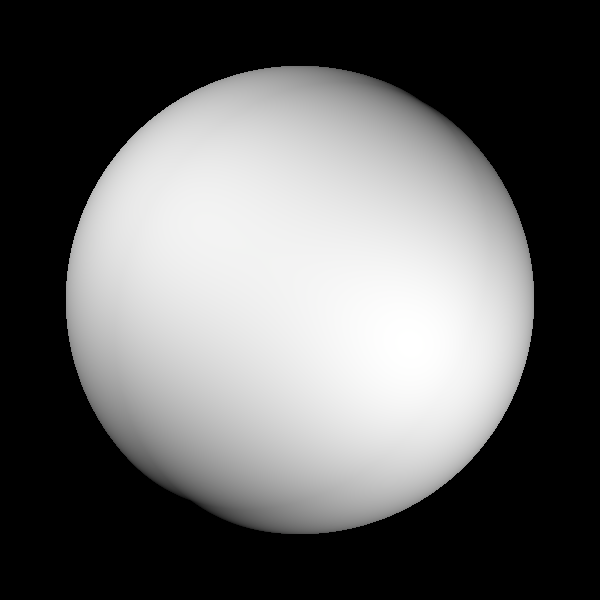
\includegraphics[width=\linewidth]{figures/image_A.png}\caption{image\_A}
\end{subfigure}\hfill
\begin{subfigure}{0.32\textwidth}\centering
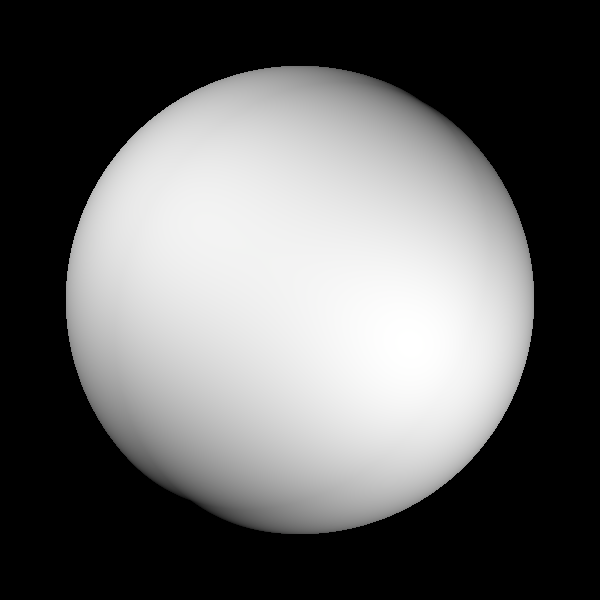
\includegraphics[width=\linewidth]{figures/image_1.png}\caption{image\_1, пересчёт}
\end{subfigure}\hfill
\begin{subfigure}{0.32\textwidth}\centering
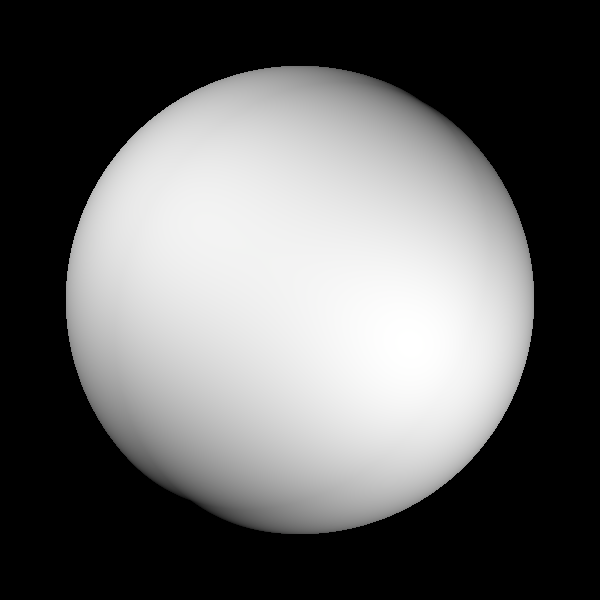
\includegraphics[width=\linewidth]{figures/image_2.png}\caption{image\_2, пересчёт}
\end{subfigure}
\caption{Три пути при одинаковой белой сфере, учебном освещении и экспозиции}
\end{figure}
\begin{table}[H]\centering\small
\caption{Отличие A при одинаковой белой сфере и модели учебника}
\begin{tabular}{@{}lrrr@{}}\toprule Пара & RMSE абсолютного RGB & MAE PNG & Max PNG\\\midrule
A / image\_1 & 4.821e-15 & 0.000000 & 0 \\
A / image\_2 & 2.582e-15 & 0.000000 & 0 \\
\bottomrule\end{tabular}\end{table}
При $k_d=1$ метамерные спектры дают совпадающие изображения, хотя энергетическая яркость различается. Совпадение не означает восстановления истинного D65.

Фактически сохранённые файлы работы 3 использовали зелёный материал, другую формулу освещения и кусочное кодирование sRGB. В \code{results/image_1.png} и \code{image_2.png} сохранён контролируемый пересчёт двух последовательностей работы 3 с белым материалом и учебной формулой. Исходные файлы оставлены в \code{reference_lab3} и показаны отдельно.
\begin{figure}[H]\centering
\begin{subfigure}{0.31\textwidth}\centering
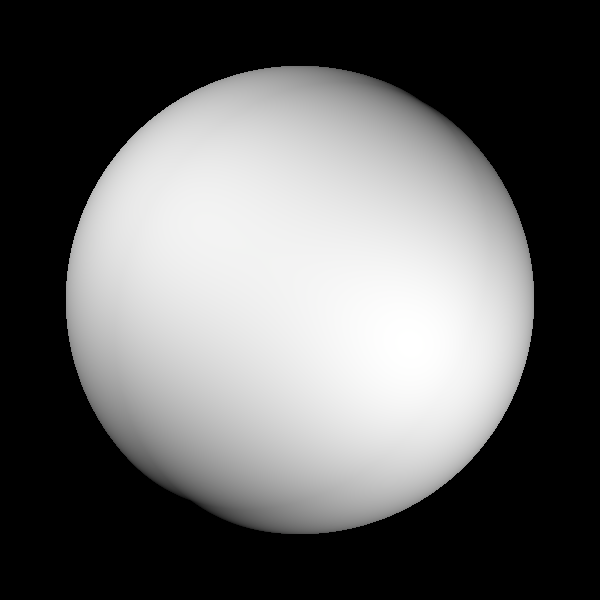
\includegraphics[width=\linewidth]{figures/image_A.png}\caption{A, белая сфера}
\end{subfigure}\hfill
\begin{subfigure}{0.31\textwidth}\centering
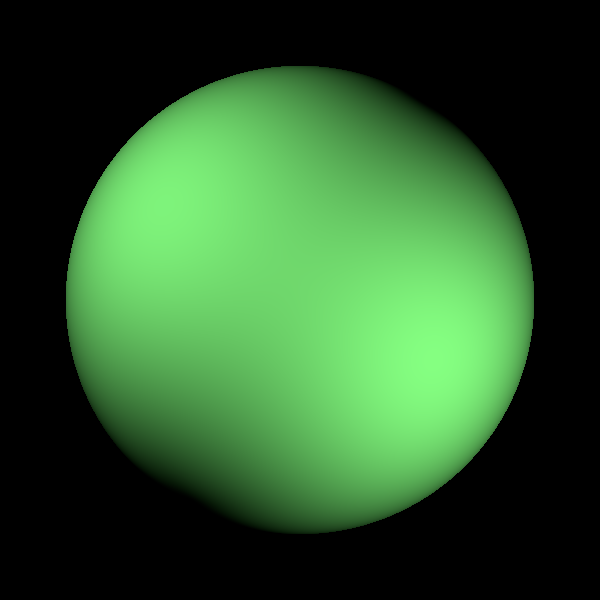
\includegraphics[width=\linewidth]{figures/original_lab3_1.png}\caption{Сохранённый Lab3 image\_1}
\end{subfigure}\hfill
\begin{subfigure}{0.31\textwidth}\centering
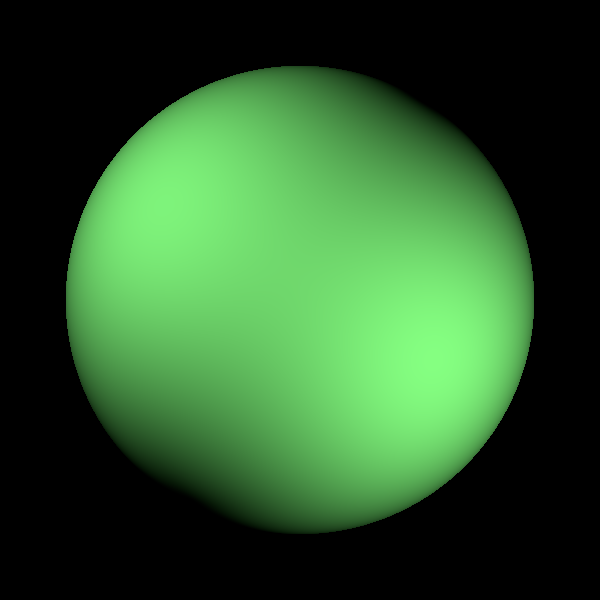
\includegraphics[width=\linewidth]{figures/original_lab3_2.png}\caption{Сохранённый Lab3 image\_2}
\end{subfigure}
\caption{Отдельное сравнение с фактическими PNG работы 3}
\end{figure}
\begin{table}[H]\centering\small
\caption{Прямое сравнение сохранённых PNG при разных условиях}
\begin{tabular}{@{}lrr@{}}\toprule Пара & MAE (весь кадр) & Max\\\midrule
A / original Lab3 image\_1 & 41.069551 & 136 \\
A / original Lab3 image\_2 & 41.069551 & 136 \\
\bottomrule\end{tabular}\end{table}

\subsection{Три точки и экстремумы}
Яркость в контрольных точках вычислена по формулам, а не по ближайшему пикселю. Все точки видимы и лежат на сфере.
\begin{table}[H]\centering\footnotesize
\caption{Контрольные точки изображения A}
\begin{tabular}{@{}lrrr rr@{}}\toprule Точка & x, мм & y, мм & z, мм & $L_e$, Вт/(м$^2$ ср) & $L_v$, кд/м$^2$\\\midrule
P1 & 0 & 0 & 950 & 17.5502459 & 5719.5448387 \\
P2 & -210 & 0 & 880 & 14.1445246 & 4609.6358595 \\
P3 & 210 & 0 & 880 & 17.1218663 & 5579.9378874 \\
\bottomrule\end{tabular}\end{table}
\begin{table}[H]\centering\small
\caption{Экстремумы изображения A, фон исключён}
\begin{tabular}{@{}lrr@{}}\toprule Область и величина & Минимум & Максимум\\\midrule
Видимые пиксели, $L_e$ & 0.0000000 & 19.3582805 \\
Видимые пиксели, $L_v$ & 0.0000000 & 6308.7750271 \\
Вся сфера, $L_e$ & 0.0000000 & 19.3573313 \\
Вся сфера, $L_v$ & 0.0000000 & 6308.4656971 \\
\bottomrule\end{tabular}\end{table}
Фон исключён маской. Нулевой минимум относится к неосвещённой поверхности. Экстремумы всей сферы оценены на сетке 181 полярного угла и 360 азимутов. Это дискретные оценки, а не доказанные непрерывные экстремумы.

\section{Программа и проверка}
Единственный пакет \code{lab4_spectrum} содержит модули \code{reconstruction.py} для системы трёх базисов, \code{experiment.py} для расчёта и сравнения, \code{output.py} для экспорта и \code{gui.py} с классом App. Подпакет \code{core} отвечает за геометрию, интегрирование и рендеринг. Корневой \code{lab4.py} --- только точка запуска. Прежний решатель, альтернативный косинусный режим и неиспользуемые загрузчики сцен удалены.

GUI сохраняет структуру работы 3: слева параметры, справа изображения, спектрограммы с таблицей и абсолютные величины. Расчёт идёт в рабочем потоке, обновление Tk --- в основном. Экспорт сохраняет последний рассчитанный результат.
\IfFileExists{figures/gui.png}{\begin{figure}[H]\centering
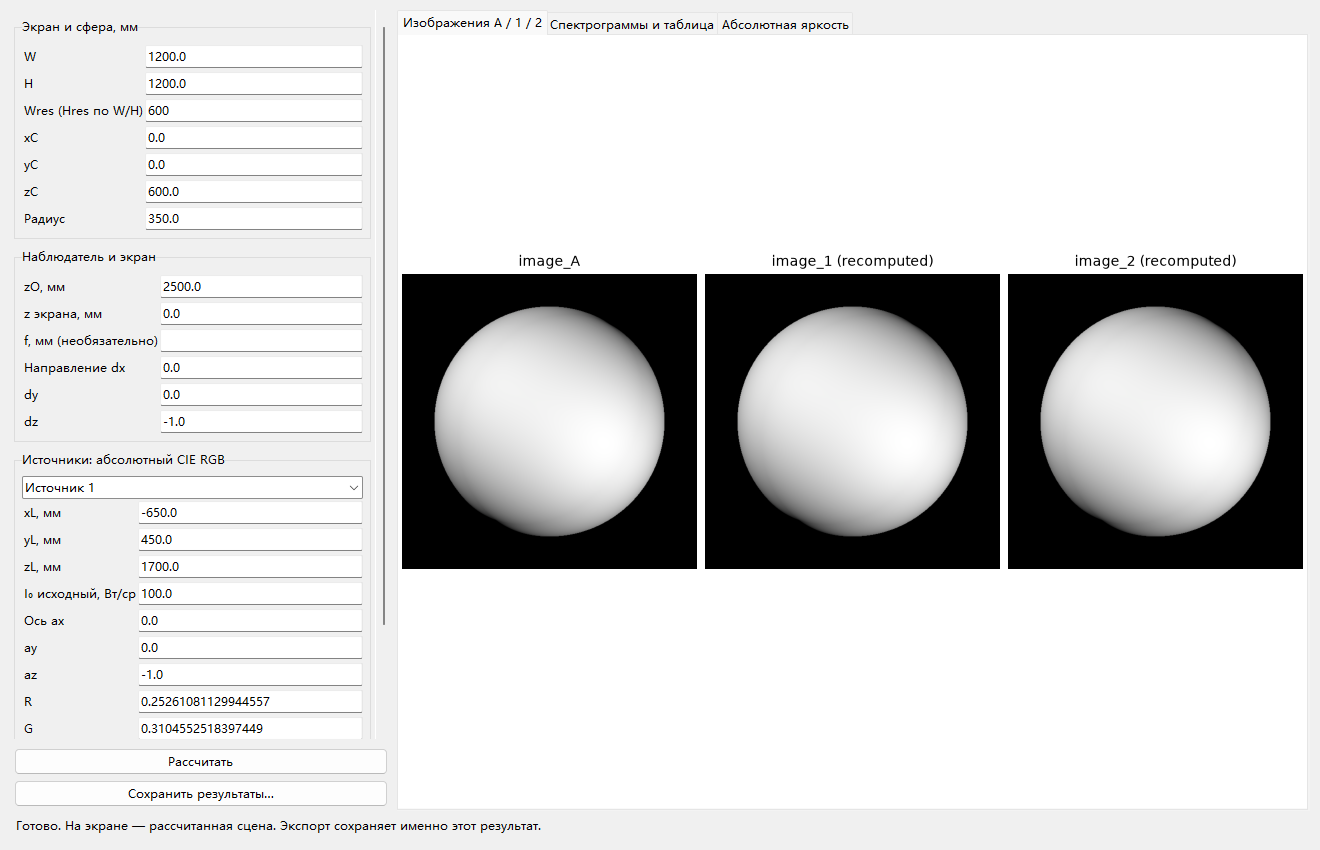
\includegraphics[width=\textwidth]{figures/gui.png}\caption{Интерфейс новой версии}
\end{figure}}{}
Пять проверок охватывают цветовое соответствие, линейность масштаба, известную комбинацию трёх базисов, неверные данные, отсутствие повторной нормировки энергии, независимый аналитический расчёт яркости в переднем полюсе, файлы и реальный цикл Tk с расчётом и экспортом. Тестовый размер --- $200\times200$, результаты отчёта отдельно получены при $600\times600$.

Запуск: \code{python lab4.py}. Без окна: \code{python -m lab4_spectrum --no-gui}. Проверка: \code{python test_lab4.py}. Отчёт написан на LaTeX, компилятор XeLaTeX. PNG, CSV, JSON и абсолютный спектральный массив NPZ приложены.

\section{Выводы}
Реализована учебная последовательность RGB $\to$ XYZ $\to$ три базовых спектра $\to$ решение системы $3\times3$ $\to$ спектральное изображение. Основа --- интегральное определение цвета и закон аддитивности. Освещение вычисляется по ламбертовской формуле учебника с одним приёмным косинусом.

Метамер сохраняет цвет D65, но имеет другую форму и интегральную энергию. Повторная нормировка изменила бы заданные цветовые координаты. При белом материале мониторные изображения трёх путей совпадают, что согласуется с метамерией. Приведены три абсолютные яркости и дискретные экстремумы. Фактически сохранённые результаты работы 3 отделены от контролируемого пересчёта.

\begin{thebibliography}{9}
\bibitem{book} Жданов Д.Д., Потемин И.С., Жданов А.Д. Теоретические основы компьютерной графики и вычислительной оптики. Санкт-Петербург, 2023. \code{Lecture/3281.pdf}. С.~47, 64--70, 77.
\bibitem{lecture4} Игнатенко А. Цветовая температура. Точка белого. Адаптация. Спектр из цвета. Лекция 4, 16 марта 2011. \code{mis_lect04_11.pdf}. С.~35--42 PDF.
\bibitem{lectures} Игнатенко А. Машинное представление цвета. Подбор цветов. Лекция 3. Гамма-коррекция. Лекция 5. \code{mis_lect03_11.pdf}, \code{mis_lect05_11.pdf}.
\bibitem{rays} Игнатенко А. Трассировка лучей. Алгоритмы поиска пересечений. Лекция 11. \code{mis_lect11_11.pdf}. С.~34--35 PDF.
\bibitem{assignment} Задание лабораторной работы 4. \code{АКГ_лр4.docx}.
\bibitem{cie} CIE. Standard illuminant D65. DOI: \href{https://doi.org/10.25039/CIE.DS.hjfjmt59}{10.25039/CIE.DS.hjfjmt59}. Данные D65 унаследованы из работы 3, лицензия CC BY-SA 4.0.
\end{thebibliography}
\end{document}

